% Create well-known link to this spot for HTML version
\ifpdf
\else
\HCode{<a name='DUCC_OVERVIEW'></a>}
\fi
\chapter{DUCC Overview}

    \section{What is DUCC?}

    DUCC stands for Distributed UIMA Cluster Computing. DUCC is a cluster management system
    providing tooling, management, and scheduling facilities to automate the scale-out of
    applications written to the UIMA framework.

    Core UIMA provides a generalized framework for applications that process unstructured
    information such as human language, but does not provide a scale-out mechanism. UIMA-AS provides
    a scale-out mechanism to distribute UIMA pipelines over a cluster of computing resources, but
    does not provide job or cluster management of the resources. DUCC defines a formal job model
    that closely maps to a standard UIMA pipeline. Around this job model DUCC provides cluster
    management services to automate the scale-out of UIMA pipelines over computing clusters.

    \section{DUCC Job Model}

    The Job Model defines the steps necessary to scale-up a UIMA pipeline using DUCC.  The goal of
    DUCC is to allow the application logic to be unchanged.

    The DUCC Job model consists of standard UIMA components: a Collection Reader (CR), a CAS
    Multiplier (CM), application logic as implemented one or more Analysis Engines (AE), and a CAS
    Consumer (CC).  In theory, any CR, or CM will work with DUCC, but DUCC is all about scale-out.  In
    order to achieve good scale-out these components must be constructed in a specific way.

    The Collection Reader builds input CASs and forwards them to the UIMA pipelines.  In the DUCC
    model, the CR is run in a process separate from the rest of the pipeline. In face, in all but the
    smallest clusters it is run on a different physical machine than the rest of the pipeline.  To
    achieve scalability, the CR must create very small CASs that do not contain application data,
    but which contain references to data; for instance, file names.  Ideally, the CR should be
    runnable in a process not much larger than the smallest Java virtual machine.  Later sections
    demonstrate methods for achieving this.

    Each pipeline must contain at least one CAS Multiplier which receives the CASs from the CR.  The
    CMs encapsulate the knowledge of how to receive the data references in the small CASs received
    from the CRs and deliver the referenced data to the application pipeline.  DUCC packages the CM,
    AE(s), and CM into a single process, multiple instances of which are then deployed over the
    cluster.

    DUCC does not provide any mechanism for receiving output CASs.  Each application must
    supply its own CAS Consumer which serializes the output of the Analytic Engines for 
    consumption by other entities (as serialized CASs, perhaps, or as some other form of
    data, depending on what the other entities are.).

    A DUCC job therefore consists of a small specification containing the following items:
    
    \begin{itemize}
      \item The name of a resource containing the CR descriptor.
      \item The name of a resource containing the CM descriptor.
      \item The name of a resource containing the AE descriptor.
      \item The name of a resource containing the CC descriptor.
      \item Other information required to parametrize the above and identify the job
        such as log directory, working directory, desired scale-out, etc.  These are
        described in detail in subsequent sections.
    \end{itemize}

    On job submission, DUCC examines the job specification and automatically creates a scaled-out
    UIMA-AS service with a single process executing the CR as a UIMA-AS client and and as many
    processes as possible executing the combined CM, AE, and CC pipeline as UIMA-AS service
    instances.

    DUCC provides other facilities in support of scale-out:
    \begin{itemize}
      \item The ability to reserve all or part of a node in the cluster.
      \item Automated management of services required in support of jobs.
      \item The ability to schedule and execute arbitrary processes on nodes in the
        cluster.
      \item Debugging tools and support.
      \item A web server to display and manage work and cluster status.
      \item A CLI and a Java API to support the above.
    \end{itemize}
    
    \section{DUCC From UIMA to Full Scale-out}

    In this section we demonstrate the progression of a simple UIMA pipeline to a fully
    scaled-out job running under DUCC.

    \paragraph{UIMA Pipelines}
    A normal UIMA pipeline
    contains a Collection Reader, one or more Analysis Engines connected in a pipeline, and a CAS
    Consumer as shown in \hyperref[fig:UIMA-pipeline]{Figure ~\ref{fig:UIMA-pipeline}}.

    \begin{figure}[H]
      \centering
      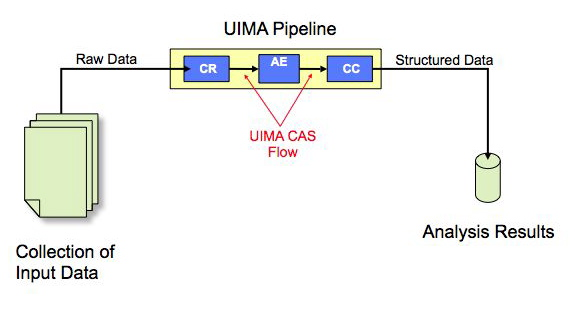
\includegraphics[bb=0 0 575 310, width=5.5in]{images/uima-pipeline.jpg}
      \caption{Standard UIMA Pipeline}
      \label{fig:UIMA-pipeline}
    \end{figure}

    \paragraph{UIMA-AS  Scaled Pipeline}
    With UIMA-AS the CR is separated into a discrete process and a CAS Multiplier is introduced 
    into the analytic pipeline as an interface between the CR and the pipeline, as shown in
    \hyperref[fig:UIMA-AS-pipeline]{Figure ~\ref{fig:UIMA-AS-pipeline}} below.
    Multiple analytic pipelines are serviced by the 
    CR and are scaled-out over a computing cluster.  The difficulty with this model is that each
    user is individually responsible for finding and scheduling computing nodes, installing
    communication software such as ActiveMQ, and generally managing the distributed job and
    associated hardware.

    \begin{figure}[H]
      \centering
      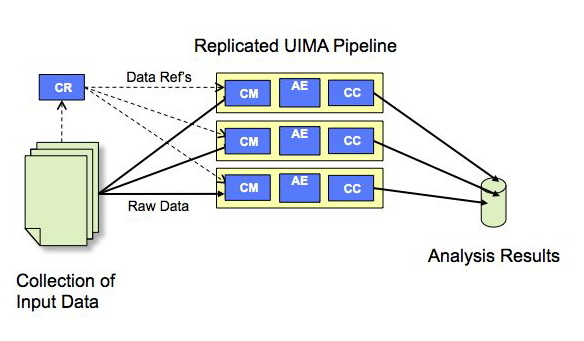
\includegraphics[bb=0 0 584 341, width=5.5in]{images/uima-as-pipeline.jpg}
      \caption{UIMA Pipeline As Scaled by UIMA-AS}
      \label{fig:UIMA-AS-pipeline}
    \end{figure}

    \paragraph{UIMA-AS Pipeline Scaled By DUCC}
    DUCC is a UIMA and  UIMA-AS-aware cluster manager.  To scale out work under DUCC the developer
    tells DUCC what the parts of the application are, and DUCC does the work to build the
    scale-out via UIMA/AS, to find and schedule resources, to deploy the parts of the application
    over the cluster, and to manage the jobs while it executes.

    On job submission, the DUCC Command Line Interface (CLI) inspects the XML defining the analytic
    and generates a UIMA-AS Deployment Descriptor (DD).  The DD establishes some number of pipeline
    threads per process (as indicated in the DUCC job parameters), and generates job-unique queues.

    Under DUCC, the Collection Reader is executed in a process called the Job Driver (or JD). The 
    analytic pipelines are executed in one or more processes called Job Processes (or JPs). The JD 
    process provides a thin wrapper over the CR to enable communication with DUCC.  The JD uses the
    CR to implement a UIMA-AS client delivering CASs to the multiple (scaled-out) pipelines, 
    shown in \hyperref[fig:UIMA-AS-pipeline-DUCC]{Figure ~\ref{fig:UIMA-AS-pipeline-DUCC}} below.

    \begin{figure}[H]
      \centering
      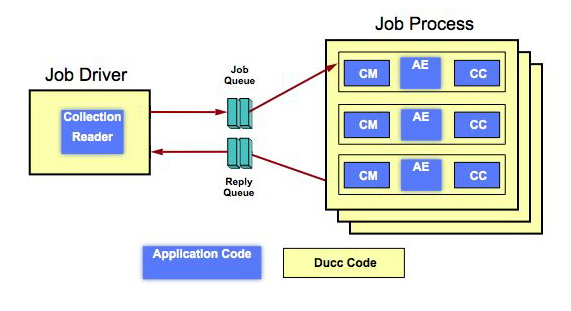
\includegraphics[bb=0 0 571 311, width=5.5in]{images/ducc-sequential.jpg}
      \caption{UIMA Pipeline As Automatically Scaled Out By DUCC\label{fig:UIMA-AS-pipeline-DUCC}}
    \end{figure}

    \paragraph{UIMA-AS Pipeline with User-Supplied DD Scaled By DUCC}

    Application programmers may supply their own Deployment Descriptors to control intra-process
    threading and scale-out.  If a DD is supplied in the job parameters, DUCC will use this instead
    of generating one as depicted in \hyperref[fig:UIMA-AS-pipeline-DUCC-DD]{Figure ~\ref{fig:UIMA-AS-pipeline-DUCC-DD}} below.

    \begin{figure}[H]
      \centering
      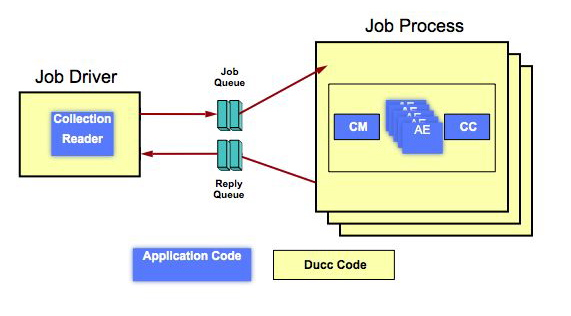
\includegraphics[bb=0 0 571 316,width=5.5in]{images/ducc-parallel.jpg}
      \caption{UIMA Pipeline With User-Supplied DD as Automatically Scaled Out By DUCC}
      \label{fig:UIMA-AS-pipeline-DUCC-DD}
    \end{figure}

  
    \section{Error Management }
    DUCC provides a number of facilities to assist error management:
    
    \begin{itemize}
      \item DUCC uses the UIMA-AS error-handling facilities to reflect errors from the Job Processes
        to the Job Drivers. The JD wrappers implement logic to enforce error thresholds, to identify
        and log errors, and to reflect job problems in the DUCC Web Server.  All error thresholds are
        configurable globally, and on a per-job basis.

      \item Error and timeout thresholds are implemented for both the initialization phase of a pipeline
        and the execution phase.
    
      \item Retry-after-error is supported: if a process has a failure on some CAS after
        initialization is successful, the process is terminated and the CAS retried, up to some
        configurable threshold.

      \item DUCC insures that processes can successfully initialize before fully scaling out a job,
        to insure a cluster is not overwhelmed with errant processes.
      \end{itemize}
      
    \section{Cluster and Job Management}
    DUCC provides significant support for managing multiple jobs and multiple users in a distributed cluster:

    \begin{description}
        \item[Multiple User Support] DUCC runs all work under the identity of the submitting user to
          provide security and privacy for each user and job. Logs are written with the
          user's credentials into the user's file space designated at job submission.

        \item[Fair-Share Scheduling] DUCC provides a Fair-Share scheduler to equitably share
          resources among multiple users.  The scheduler also supports semi-permanent reservation of
          full or partial machines.

        \item[Service Management] DUCC provides a Service Manager capable of automatically starting, stopping, and
          otherwise managing and querying services in support of jobs.

        \item[Job Lifetime Management and Orchestration] DUCC includes an Orchestrator to manage the
          lifetimes of all entities in the system.
          
        \item[DUCC Agents] DUCC Agents manage each node's local resources and all
          processes started by DUCC. Each node in a cluster has exactly one Agent. The Agent
          \begin{itemize}
            \item Monitors and reports node capabilities (memory, etc) and performance data (CPU busy,
              swap, etc).
            \item Starts and stops all processes on behalf of users.
            \item Patrols the node for ``foreign'' (non-DUCC) processes, reporting them to the
              Web Server, and optionally reaping them.
            \item Insures job processes to not exceed their declared memory requirements
              through the use of Linux Cgroups.
          \end{itemize}

        \item[DUCC Web server] DUCC  provides a web server displaying all aspects of the system:
          \begin{itemize}
              \item All jobs in the system, their current state, resource usage, etc.
                
              \item All reserved resources and associated information (owner, etc.),
                including the ability to request and cancel reservations.
                
              \item All services, including the ability to start, stop, and modify
                service definitions.
                
              \item All nodes in the system and their status, usage, etc. 
                                
              \item The status of all DUCC management processes.  

              \item Access to documentation.
          \end{itemize}


        \item[Cluster Management Support] DUCC provides rich scripting support to:
          \begin{itemize}
              \item Start, stop, and query full DUCC systems.
 
              \item Start, stop, and quiesce individual DUCC components.
 
              \item Add and delete nodes from the DUCC system.
 
              \item Discover DUCC processes (e.g. after partial failures).
 
              \item Find and kill errant job processes belonging to individual users.
                
              \item Monitor and display inter-DUCC messages.
          \end{itemize}
      \end{description}

